\documentclass[11pt]{article}
\usepackage{graphicx}
\usepackage{float}
\usepackage{amsmath}
\usepackage{amsfonts}
\usepackage[brazilian]{babel}
\usepackage[utf8]{inputenc}
\usepackage[backend=biber]{biblatex}
\usepackage{csquotes}
%\usepackage{docmute}
\usepackage{array}
\usepackage{geometry}
\usepackage[T1]{fontenc}
\addbibresource{plano_de_pesquisa.bib}

\newcommand{\fromeng}[1]{\footnote{do inglês: \textit{#1}}}
\newcommand{\tit}[1]{\textit{#1}}
\newcommand{\tbf}[1]{\textbf{#1}}
\newcommand{\ttt}[1]{\texttt{#1}}

\newcolumntype{C}[1]{>{\centering\let\newline\\\arraybackslash\hspace{0pt}}m{#1}}

\begin{document}

\begin{titlepage}
	\centering
	{\scshape\Large Projeto de pesquisa\par}
	\vspace{1.5cm}
	{\huge \bfseries Atenção visual para sistemas robóticos
        com \tit{Deep Learning}\par}
	\vspace{1cm}
	{\itshape Aluno: Erik de Godoy Perillo\par}
	{\itshape Orientadora: Profa. Dra. Esther Luna Colombini\par}
	\vspace{0.5cm}
	\begin{abstract}
        A informação visual é um elemento-chave no processo de entender
        o ambiente em que um ser se encontra.
        Para sistemas robóticos isso também é verdade.
		No entanto, a alta dimensionalidade dos dados captados por câmeras
		usadas para este fim é em geral problemática, muitas vezes havendo
		redundância e irrelevância de informação.
		Nos seres humanos este filtro sensorial é realizado pela Atenção.
		Neste contexto, este projeto propõe a aplicação de
        \tit{Deep Learning} para a obtenção de sistemas de saliência visual
        para sistemas robóticos.
        Este trabalho dá continuidade ao trabalho anterior, onde as técnicas
        mais recentes para abordar o problema foram avaliadas, focando-se em um
        novo modelo competitivo com os atuais e otimizado
        para o domínio de robótica.
        Neste trabalho, visamos a extensão do modelo para fluxos contínuos de
        imagem, representados por vídeo.
	\end{abstract}
	\vfill
	Universidade Estadual de Campinas
	\vfill
	{\large \today\par}
\end{titlepage}

\newpage

\section{Introdução}
\paragraph{}
Um desafio ainda em aberto na robótica é a concepção de robôs que lidam com
o imprevisível, reagindo de forma apropriada às mais diversas situações
do mundo real.
Sistemas que interagem com o ambiente, objetos e pessoas
com uma variedade de maneiras semelhante à nossa têm o potencial de ser
usados em diversar aplicações domésticas, industriais e em agricultura,
sendo assim muito benéficos para a sociedade.

Um dos componentes fundamentais para tais sistemas de navegação autônoma é seu
sistema visual.
Dentre os diversos sub-problemas relacionados a se obter
tal sistema, está o da saliência: dada uma imagem, qual região é mais
relevante e como tal região varia no tempo?

O problema da saliência visual tem sido atacado de diversas maneiras há anos.
Recentemente, com o progresso do \tit{Deep Learning}, diversos novos modelos
e técnicas apareceram com desempenho consideravelmente superior
~\cite{ref:mit300-bm}.
Modelos atuais, entretanto, focam apenas no problema da saliência visual
para imagens estáticas.
Em fluxos contínuos de imagens, ou seja, vídeos, há efeitos que não existem
para imagens fixas que mudam o foco da atenção.

\subsection{Motivação}
Um problema de sensores usados para tarefas mais complexas de navegação
em geral
é que o volume de dados a ser processado pode ser demasiadamente grande.
Para um robô que interage continuamente com o ambiente, é improvável que em
todos os instantes  toda informação proveniente de seus sensores seja
processada ou mesmo necessária.
Isso é especialmente crítico para sistemas robóticos que precisam de respostas
rápidas para interagir com o ambiente em que estão inseridos.

\subsection{Saliência visual}
Saliência visual pode ser definida como uma região visual em que se dá
foco para um maior trabalho cognitivo em um certo momento.~\cite{ref:fit}
Com base no comportamento de humanos, modelos computacionais que simulam
a atenção o fazem geralmente por meio de mapas de saliência, que são
computados para uma certa imagem.
A figura~\ref{fig:sal-map} exemplifica um mapa.
Pixels com valores altos (brancos) representam áreas de alta saliência.

\begin{figure}[H]
    \centering
    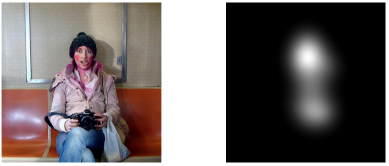
\includegraphics[width=0.6\linewidth]{imgs/sal_map_1.png}
    \caption{Exemplo de mapa de saliência para uma certa imagem
    ~\cite{ref:salicon}.}
    \label{fig:sal-map}
\end{figure}

Diversos métodos para geração de tais mapas foram propostos ao longo dos anos.
Vocus~\cite{ref:vocus}, por exemplo, é um modelo que leva em consideração
aspectos globais da imagem e contraste em relação a fatores
como cor, direção, luminância em diversas dimensões.

A introdução de \tit{Deep Learning} à área de saliência visual
possibilitou mapas com desempenho
superior em geral a modelos antigos, com a vantagem intrínseca da técnica que
é a geração automática de \tit{features} a serem extraídas.
Modelos como \tit{Salicon}~\cite{ref:salicon}, \tit{DeepFix}~\cite{ref:deepfix}
e \tit{Salnet}~\cite{ref:shallow-deep} têm desempenho superior aos modelos
atencionais tradicionais em todas as métricas
estabelecidas pelo \tit{MIT Saliency Benchmark}~\cite{ref:mit300-bm}.

Considerando que nosso trabalho tem como foco usar modelos atencionais para
agentes robóticos exploratórios~\cite{ref:previous-proposal},
os modelos atuais apresentam dois problemas
fundamentais: a) eles são demasiadamente pesados computacionalmente,
dificultando a implementação em um sistema embarcado, e b) não são
feitos para fluxos de imagens, ou seja, vídeos, não levando em
consideração efeitos que acontecem neste cenário como inibição de retorno
~\cite{ref:esther-thesis}.

\section{Objetivos}
Neste contexto, este projeto tem por objetivo construir um modelo de saliência
visual que seja mais eficiente computacionalmente
(sem muita perda de desempenho) e que simule o comportamento de humanos
com relação à variação espacial do foco atencional no tempo em fluxos
contínuos de imagens.
Mais especificamente, objetivamos:

\begin{itemize}
	\item Obtenção de uma arquitetura de rede neural artificial otimizada para
        a extração de mapas de saliência da imagem e que seja relativamente
        eficiente computacionalmente;
	\item Adaptação da rede obtida para vídeo, com mecanismos extras
        que simulem o comportamento humano padrão;
	\item Implementação do sistema em uma plataforma de testes robótica
        para sua avaliação.
\end{itemize}

\section{Materiais e Métodos}
\subsection{Modelo atual}
As arquiteturas com melhor desempenho médio nas métricas do
\tit{MIT Saliency Benchmark} têm um grande número de camadas de convolução.
Dentre \tit{Salnet, DeepFix, Salicon}, as três usam transferência de
aprendizado da já treinada rede \tit{VGG-16}~\cite{ref:vgg-16}.
Tal rede chega a ter camadas de convolução com 512 filtros de dimensões 3x3.
Os espaços de cor dos três modelos analisados são RGB e a normalização dos
dados nos modelos é feita por todo o dataset.

O modelo desenvolvido por nós (figura~\ref{fig:att-deep-model})
usa um número consideravelmente menor de
parâmetros: são 6 camadas de convolução, mas o total dos filtros de todas
as camadas é de 209. O espaço de cor utilizado foi o LAB, pois há indícios
que este seja um espaço de cor que melhor representa o sistema
visual humano~\cite{ref:vocus}.
A normalização dos dados foi feita por imagem
individualmente, pois supõe-se que no contexto da saliência, o que mais
importa é a relação dos pixels em um contexto global da imagem.
O modelo é treinado com um conjunto de dados obtido pela mesclagem do
\tit{Salicon}~\cite{ref:salicon-dataset},
\tit{MIT-1003}~\cite{ref:judd-1003-dataset}
\tit{CAT-2000}~\cite{ref:cat-2000-dataset}.
A figura~\ref{fig:att-deep-pred} mostra um mapa de saliência produzido
pelo modelo atual.

\begin{figure}[H]
    \hspace*{-0.5in}
    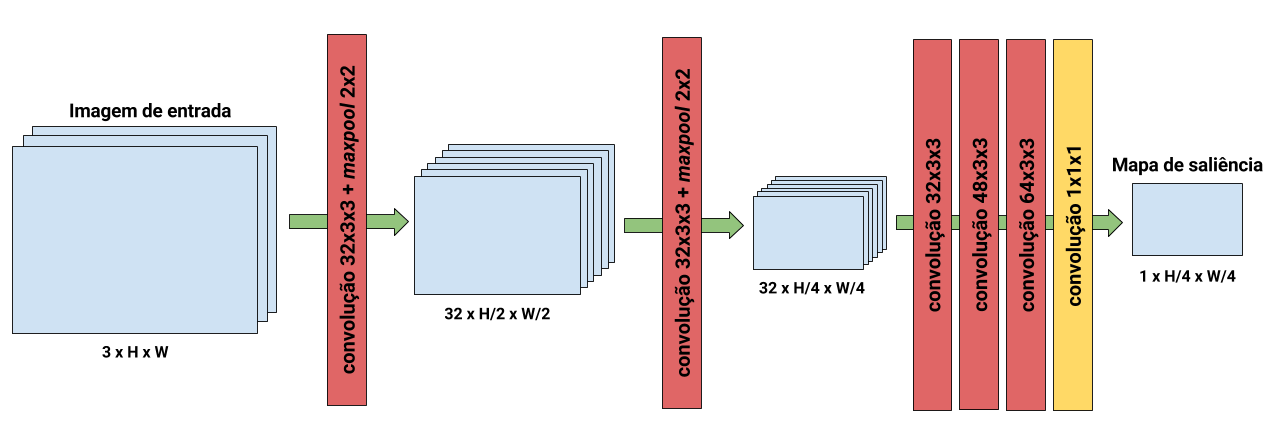
\includegraphics[width=1.2\linewidth]{imgs/att_deep.png}
    \caption{Arquitetura do modelo proposto atualmente~\cite{ref:att-deep}.}
    \label{fig:att-deep-model}
\end{figure}

\begin{figure}[H]
    \centering
    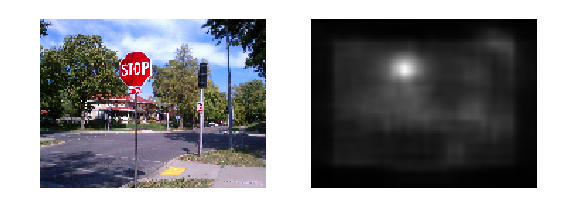
\includegraphics[width=0.7\linewidth]{imgs/our.png}
    \caption{Predição de saliência do modelo atual para uma imagem.}
    \label{fig:att-deep-pred}
\end{figure}

O modelo ainda encontra-se em estágio de desenvolvimento, mas já consegue-se
obter 0.6 na métrica \tit{Coefficient of Correlation} (CC), que é considerada
uma boa métrica que penaliza tanto falsos positivos quanto
negativos~\cite{ref:metrics}.
Tal número foi obtido em um conjunto separado de testes que não foi visto
pelo modelo durante o treinamento.
Ainda não há dados para o conjunto utilizado no \tit{MIT Saliency Benchmark},
mas o número obtido fica comparável a modelos como o
\tit{Salnet}.

\begin{table}[H]
    \centering
    \caption{Resultados de modelos no \tit{MIT Saliency benchmark}~\cite{ref:mit300-bm}.}
    \begin{tabular}{|c|c|c|c|c|c|c|c|c|}
        \hline
        \tbf{Modelo/Métrica} & \tbf{Similarity} & \tbf{CC}
            & \tbf{AUC Judd} & \tbf{NSS} & \tbf{EMD}\\
        \hline
        DeepFix~\cite{ref:deepfix} & \tbf{0.67} & \tbf{0.78} &
            \tbf{0.87} & \tbf{2.26} & \tbf{2.04}\\
        \hline
        SALICON~\cite{ref:salicon} & 0.60 & 0.74 &
            \tbf{0.87} & 2.12 & 2.62\\
        \hline
        ML-Net~\cite{ref:mlnet} & 0.59 & 0.67 &  0.85 & 2.05 & 2.63\\
        \hline
        Deep Convnet~\cite{ref:shallow-deep} & 0.52 & 0.58 &  0.83 &
            1.51 & 3.31\\
        %\hline
        %BMS & 0.51 & 0.55 & 0.65 & 0.82 & 0.83 & 1.41 & 3.35 & 0.60\\
        %\hline
        %Deep Gaze 2 & 0.46 & 0.51 & \tbf{0.76} & \tbf{0.86} & \tbf{0.87} & 1.29
        %    & 4.00 & 0.61\\
        %\hline
        %Mr-CNN & 0.48 & 0.48 & 0.69 & 0.75 & 0.79 & 1.37 & 3.71 & 0.54\\
        \hline
        Shallow Convnet~\cite{ref:shallow-deep} & 0.46 & 0.53 &  0.80
            & 1.47 & 3.99\\
        %\hline
        %GBVS & 0.48 & 0.48 & 0.63 & 0.80 & 0.81 & 1.24 & 3.51 & 0.54\\
        %\hline
        %Rare 2012 Improved & 0.46 & 0.42 & 0.67 & 0.75 & 0.77 & 1.34 & 3.74 &
        %    0.51\\
        %\hline
        %Judd & 0.42 & 0.47 & 0.60 & 0.80 & 0.81 & 1.18 & 4.45 & 0.48\\
        %\hline
        %eDN & 0.41 & 0.45 & 0.62 & 0.81 & 0.82 & 1.14 & 4.56 & 0.47\\
        \hline
    \end{tabular}
\end{table}

\subsection{Extensão para vídeos}
O modelo atualmente sendo trabalhado ainda precisa de refinamento e melhor
treinamento, que será possível graças à
obtenção recente de uma plataforma específica para treinamento da rede,
isso será possível em breve.
Após um refinamento, uma extensão para vídeos será feita.
O foco atencional depende de diversos outros fatores além do \tit{frame} atual
~\cite{ref:esther-thesis} e espera-se incorporar tais fatores no modelo novo.
Para treinamento, há conjuntos de dados como
\tit{Coutrot Database 1} e
\tit{SAVAM}~\cite{ref:videos}.

\subsection{Plataforma de testes}
Como o foco do modelo é o uso por sistemas robóticos, planeja-se usar
um robô móvel com uma GPU \tit{NVIDIA Jetson TX1} embarcada.
O objetivo é avaliar o desempenho da obtenção das regiões de saliência
com o passar do tempo e se as escolhas de foco de região são adequadas
para auxiliar na tarefa de navegação.
Objetiva-se também verificar se o modelo é eficiente computacionalmente
o suficiente para que o processamento seja feito em uma janela de tempo
adequada.

\section{Cronograma}
Para atendimento dos objetivos propostos, serão realizadas as seguintes etapas:
\begin{itemize}
	\item FASE 1: Revisão bibliográfica.
	\item FASE 2: Preparação do ambiente computacional.
	\item FASE 3: Modelagem e otimização da rede para imagens fixas.
	\item FASE 4: Extensão da rede para vídeos.
	\item FASE 5: Implementação  e testes em plataforma robótica.
\end{itemize}

\begin{table}[H]
\centering
\setlength{\tabcolsep}{.16667em}
\begin{tabular}{|C{3cm}|c|c|c|c|c|c|c|c|c|c|c|c|}
	\hline
	Tarefa/mês & Jul & Ago & Set & Out & Nov & Dez & Jan & Fev & Mar & Abr
		& Mai & Jun \\
	\hline
	FASE 1 & x & & & & & & & & & & &\\
	\hline
	FASE 2 & x & & & & & & & & & & & \\
	\hline
	FASE 3 & & x & x & x & x & & & & & & &  \\
	\hline
	FASE 4 & & & & & x & x & x & x & x & x & &  \\
	\hline
	FASE 5 & & & & & & & & & & x & x & x \\
	\hline
\end{tabular}
\end{table}

\section{Referências}
\printbibliography

\end{document}
